\section{Резултати}

\paragraph*{} Всички резултати са измерени на 2x Intel(R) Xeon(R) CPU E5-2660 0 @ 2.20GHz (Octacore CPU) с Hyperthreading. За входни данни са използвани:
\begin{itemize}
\item брой върхове N = 24 мил.
\item брой ребра M = 196 мил.
\end{itemize}

\paragraph*{} Резултатите от отделните алгоритми могат да се видят на фигура \ref{fig::running_time}.

\subsection*{Генериране на ориентиран граф}

\paragraph*{} Генерирането е прост алгоритъм, който може лесно да бъде паралелизиран на ниво данни, поради което показва високи нива на ускорение. Основното забавяне при по-висок брой нишни се дължи на това, че някои нишки свършват работата си по-бързо от други, но това няма как да се избегне, защото трябва да изчакаме целият граф да бъде генериран преди да продължим нататъка. \\

\begin{tabular}{|c|c|c|c|}
\hline
Threads & Time (s) & $S_p$ & $E_p$\\
\hline \hline
1 & 72.08 & 1.00 & 1.00 \\
\hline
2 & 37.16 & 1.94 & 0.97 \\
\hline
3 & 22.09 & 3.26 & 1.09 \\
\hline
4 & 17.51 & 4.12 & 1.03 \\
\hline
6 & 11.17 & 6.45 & 1.08 \\
\hline
8 & 9.01 & 8.00 & 1.00 \\
\hline
10 & 7.92 & 9.10 & 0.91 \\
\hline
12 & 6.36 & 11.33 & 0.94 \\
\hline
14 & 6.06 & 11.89 & 0.85 \\
\hline
16 & 5.19 & 13.89 & 0.87 \\
\hline
20 & 5.37 & 13.42 & 0.67 \\
\hline
24 & 4.71 & 15.30 & 0.64 \\
\hline
28 & 4.4 & 16.38 & 0.59 \\
\hline
32 & 3.93 & 18.34 & 0.57 \\
\hline
\end{tabular}

\subsection*{Обхождане на графа}

\paragraph*{} Обхождането е значително по-сложно затова постига много ниско ускорение. \\

\begin{tabular}{|c|c|c|c|}
\hline
Threads & Time (s) & $S_p$ & $E_p$\\
\hline \hline
1 & 9.23 & 1.00 & 1.00 \\
\hline
2 & 9.54 & 0.97 & 0.48 \\
\hline
3 & 7.7 & 1.20 & 0.40 \\
\hline
4 & 7.3 & 1.26 & 0.32 \\
\hline
6 & 6.1 & 1.51 & 0.25 \\
\hline
8 & 5.6 & 1.65 & 0.21 \\
\hline
10 & 5.4 & 1.71 & 0.17 \\
\hline
12 & 4.95 & 1.86 & 0.16 \\
\hline
14 & 4.82 & 1.91 & 0.14 \\
\hline
16 & 4.68 & 1.97 & 0.12 \\
\hline
20 & 4.9 & 1.88 & 0.09 \\
\hline
24 & 4.89 & 1.89 & 0.08 \\
\hline
28 & 4.91 & 1.88 & 0.07 \\
\hline
32 & 4.65 & 1.98 & 0.06 \\
\hline
\end{tabular}

\subsection*{Финална оценка}

\paragraph*{} Графики на ускорението и ефикасността на цялата програма могат да се видят на фигури \ref{fig::acceleration} и \ref{fig::efficiency}. \\

\begin{tabular}{|c|c|c|c|}
\hline
Threads & Time (s) & $S_p$ & $E_p$\\
\hline \hline
1 & 81.31 & 1.00 & 1.00 \\
\hline
2 & 46.7 & 1.74 & 0.87 \\
\hline
3 & 29.79 & 2.73 & 0.91 \\
\hline
4 & 24.81 & 3.28 & 0.82 \\
\hline
6 & 17.27 & 4.71 & 0.78 \\
\hline
8 & 14.61 & 5.57 & 0.70 \\
\hline
10 & 13.32 & 6.10 & 0.61 \\
\hline
12 & 11.31 & 7.19 & 0.60 \\
\hline
14 & 10.88 & 7.47 & 0.53 \\
\hline
16 & 9.87 & 8.24 & 0.51 \\
\hline
20 & 10.27 & 7.92 & 0.40 \\
\hline
24 & 9.6 & 8.47 & 0.35 \\
\hline
28 & 9.31 & 8.73 & 0.31 \\
\hline
32 & 8.58 & 9.48 & 0.30 \\
\hline
\end{tabular}

\begin{figure}[h]
  \centering
  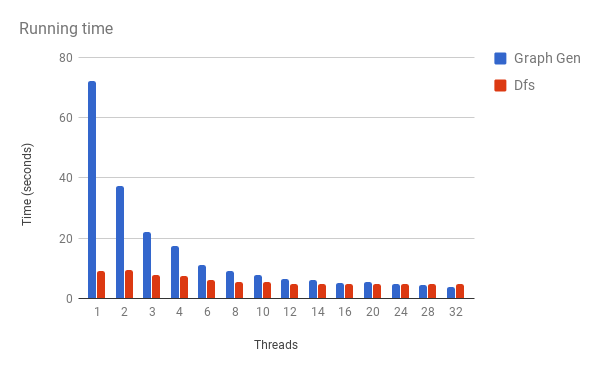
\includegraphics[width=0.8\textwidth]{resources/running_time.png}
  \caption{\label{fig::running_time} Време за изпълнение на отделните части от алгоритъма}
\end{figure}

\begin{figure}[h]
  \centering
  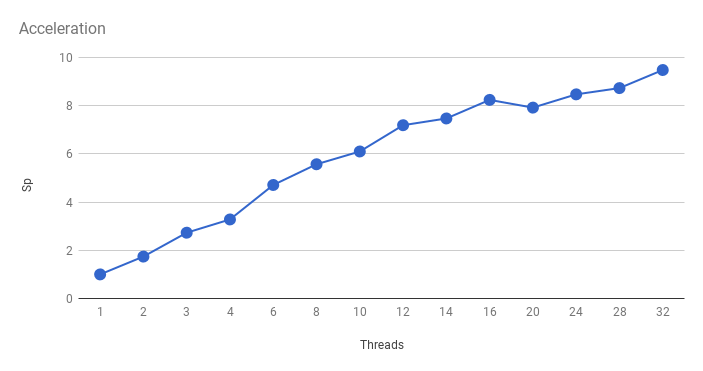
\includegraphics[width=0.8\textwidth]{resources/acceleration.png}
  \caption{\label{fig::acceleration} Графика на ускорението }
\end{figure}

\begin{figure}[h]
  \centering
  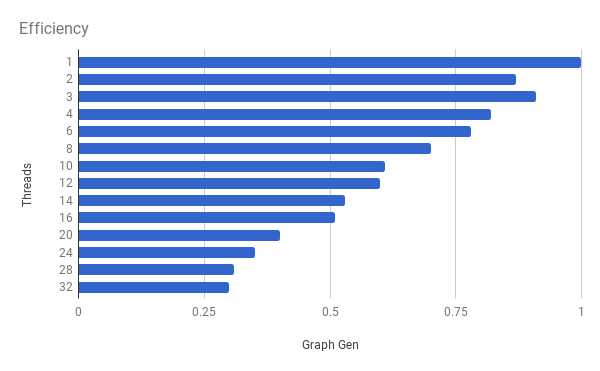
\includegraphics[width=0.8\textwidth]{resources/efficiency.png}
  \caption{\label{fig::efficiency} Графика на ефикасността }
\end{figure}
